\documentclass[a4paper,10pt]{article}


\usepackage[utf8]{inputenc}
\usepackage[T1]{fontenc}
\usepackage[francais]{babel}
\usepackage{geometry}

\usepackage{listings}
%%% basic
\usepackage{setspace}
\usepackage{titlesec}
\usepackage{titling}
\usepackage{graphicx}
\usepackage{amsmath}
\usepackage{amsthm}
\usepackage{enumitem}
\usepackage{placeins}
\usepackage{listings}
\usepackage{minted}

%%% WRITELATEX :	https://www.writelatex.com/1955619yrddkg#/4921214/

%%% clickable ref
\usepackage{hyperref}
\usepackage[all]{hypcap} %for going to the top of an image when a figure reference is clicked
\hypersetup{ % to remove red border arround links
colorlinks=false,
pdfborder={0 0 0},
}
%%% paragraph indent
\usepackage{parskip}
\setlength\parindent{15pt} % sets indent to zero
\setlength{\parskip}{1.6ex plus 0.5ex minus 0.3ex}
%%% smart space (for macros)
\usepackage{xspace}
%%% macros
\newcommand{\fref}[1]{Figure~\ref{#1}}
\newcommand{\tref}[1]{Table~\ref{#1}}
\newcommand{\sref}[1]{Section~\ref{#1}}
\newcommand{\cref}[1]{Chapter~\ref{#1}}
\newcommand{\eref}[1]{Equation~\ref{#1}}
\newcommand{\insertfigure}[4]{
\begin{figure}[ht!]
\begin{center}
\includegraphics[width=#1\textwidth]{#2}
\caption{#3}
\label{#4}
\end{center}
\end{figure}
}

%Enter your name, the portfolio problem number, and the draft number.
\title{\hrule \bigskip Projet BDA SIM \\ Base de données fédérée \bigskip \hrule}
\author{~~\\ Raphaël Baron - Guillaume Biez - Xavier Fraboulet \\ Thomas François - Damien Le Guen - Benoit Travers}

%Enter your name, the portfolio problem number, and the draft number.  This will be a heading on pages after the first page.
\markright{projet BDA SIM}



\begin{document}

%% title	
\maketitle
\thispagestyle{empty}
\newpage

%% blank page
~~\\
\thispagestyle{empty}
\newpage

%% table of contents
\tableofcontents

%%% new section
\newpage
\section{Introduction}
Avec la croissance actuelle de la quantité et des sources de données - notamment avec la progression de l'Internet des objets - l'architecture des bases de données classiques possédant un unique serveur de données central, montre progressivement ses limites. Aujourd'hui les entreprises sont de plus en plus amenées à croiser entre elles ces différentes sources de données. Il serait intéressant de pouvoir y accéder sans avoir à se soucier de leur hétérogéneité. C'est dans ce but qu'a été défini le modèle de l'architecture fédérée.

Notre présent rapport s'intéresse donc à la réalisation d'une base de données fédérée mettant l'accent sur une interface d'accès unique à des données de différentes sources. Notre philosophie ici est d'arriver à la réalisation d'une chaîne complète de transmission de requête, de l'émission de la requête à la réception de la réponse par le client. Le tout de manière simplifiée mais fonctionnelle de bout en bout.

Après avoir observé l'état de l'art actuel, nous étudierons la solution développée pour ce projet, partie par partie. Enfin, la dernière section portera sur les tests effectués pour valider le fonctionnement de notre projet.





%%% new section
\newpage
\section{Présentation}
\subsection{Définition}
Au sein d'une même entreprise, il n'est pas rare d'avoir à traiter différents types et formats de données. Y accéder indépendamment n'est pas un souci, mais dès lors qu'il est question de traiter et croiser ces sources hétérogènes, cela peut très vite virer au casse-tête. C'est pour répondre à ce type de problématique qu'a été défini le modèle d'architecture fédérée : communiquer de manière transparente avec chaque base tout en leur laissant leur autonomie. Au coeur de cette architecture, on trouve deux parties principales : 
\begin{itemize}
\item La première est le médiateur. Il joue le rôle d'interface que vient interroger l'utilisateur de la base à l'aide d'un seul et même langage. Il se charge ensuite de découper la requête et de l'envoyer aux bases concernées.
\item La seconde partie est représentée par les wrappers. Pour chaque format de données, un wrapper doit être développé pour faire le lien en entrée et en sortie avec le médiateur et la base de données correspondante. Il convertit la requête et la réponse dans les langages adéquats.
\end{itemize}

\subsection{Les contraintes de l'architecture fédérée}
Une base de données fédérée est donc une architecture visant à communiquer de manière transparente avec des sources hétérogènes et potentiellement distribuées sur plusieurs machines. Étrangement, bien que ce modèle d'architecture fédérée soit défini depuis le milieu des années 80, il n'existe toujours pas de solution universellement répandue, qu'elle soit open-source ou commerciale. Cela s'explique par plusieurs facteurs. 

Tout d'abord, la contrainte d'accéder à des données hétérogènes ne permet pas de supposer \textit{à priori} des formats nécessaires à chaque utilisateur. Ainsi, si pour certains utilisateurs le support de XML et de SQL sera amplement suffisant, d'autres réclameront le support de formats très divers, parfois non standardisés, voire spécifiquement conçu en interne par l'entreprise. Dans ce cas-là, l'utilisateur sera forcé d'écrire par lui-même un nouveau wrapper propre au format.

De la même manière, le format principal de communication à la base fédérée n'est pas nécessairement taillé à tous les scénarios d'utilisation. Si la plupart du temps, la combinaison XQuery en entrée et XML en sortie convient aux applications web courantes, qu'advient-il en cas de non-compatibilité avec  ces formats ? Le plus souvent, toute la chaîne de routage de requêtes est alors à recoder.


\subsection{Les modèles existants}
On l'a vu, l'architecture fédérée ne se prête pas à une solution définitive fournie clés-en-mains. Pourtant, certains outils existent. Parmi eux, nous nous sommes penchés sur XML Mediator de e-XMLMedia et Liquid Data de BEA.

\subsubsection{XML Mediator de e-XMLMedia}
Comme son nom l'indique, cet outil permet la création d'un médiateur pour accéder et publier des données variées au format XML. Comme le montre la \fref{fig:xmlmediator}, il dispose de plusieurs wrappers intégrés ainsi que d'interfaces permettant de créer des wrappers personnalisés.

Il dispose de plusieurs fonctionnalités intéressantes, notamment le support de requêtes XQuery distribuées et l'utilisation possible dans tout environnement de type SOAP. Il est de fait bien adapté à une implémentation pour services web.

\insertfigure{1}{E-XML.png}{Architecture du médiateur e-XML}{fig:xmlmediator}

\subsubsection{Liquid Data de BEA}
Sorti au début des années 2000, ce système permet, par l'intermédiaire d'une interface utilisateur graphique (cf. \fref{fig:liquiddata}), de définir les relations entre les données et les requêtes qui leurs seront adressées. Il permet également un accès répété aux bases en soumettant des requêtes paramétrées et de simplifier la récupération de résultats à partir d'une application web à l'aide de Liquid Data Control. Néanmoins, cette solution propriétaire vieillissante offre peu de souplesse pour intervenir dans d'autres cas d'utilisation que par accès web.

\insertfigure{0.8}{LiquidData.png}{Création d'une requête paramétrée via l'interface de Liquid Data}{fig:liquiddata}







%%%%%%%%%%%%%%%%%%%%%%%%%%%%%%%%%%%%%%%%%%
%%%%%%%%%%%%%% Solution %%%%%%%%%%%%%%%%%%
%%%%%%%%%%%%%%%%%%%%%%%%%%%%%%%%%%%%%%%%%%
%%% new section
\FloatBarrier
~~\\
\newpage
\section{Solution}

Notre choix de langage pour les requêtes s'est porté sur XQuery, et sur XML pour le format de retour. Ainsi, la base de données fédérée apparait comme une liste de fichiers XML aux yeux de l'utilisateur.


La \fref{fig:archiglo} présente l'architecture de la solution. Ces différents modules vont être présentés et détaillés dans les sections suivantes.

Par ailleurs, nous avons écrit deux wrappers afin de prendre en compte deux types de bases :
\begin{itemize}
\item base de données XML ;
\item base de données relationnelle SQLite3 (par abus de langage, nous parlerons de base de données SQL dans la suite de ce rapport).
\end{itemize}


\insertfigure{0.7}{Archi_Global.jpg}{Architecture globale de la solution}{fig:archiglo}



%%%%%%%%%%%%%%%%%%%%%%%%%%%%%%%%%%%%%%%%%%


\subsection{Médiateur}

Le médiateur a pour objectif de séparer la requête en sous-requêtes et d'assembler les résultats intermédiaires issus des sous-requêtes.

\subsubsection{Découpage de la requête}

L'utilisateur soumet à la base de données fédérée une requête XQuery susceptible de porter sur plusieurs tables appartenant à différentes bases de données.
Grâce à la classe \emph{Splitter}, la base de données fédérées est en mesure de découper la requête XQuery en de multiple sous-requêtes. 
Pour des raisons de simplicité d'implémentation, les sous-requêtes que nous avons cherché à isoler sont les morceaux du XQuery ayant la forme suivante : \emph{doc("Table")XPath}.
Ainsi, les sous-requêtes sont des requêtes de type XPath avec leur table associée. 

Une fois le découpage effectué, les sous-requêtes sont envoyées aux wrappers associés aux bonnes bases de données grâce à la table de routage.
Ce wrapper se chargera de transformer la requête XPath dans le bon langage.

Nous allons illustrer le découpage d'une requête XQuery avec l'exemple de la \fref{lst:exempleRequete}. 

\begin{figure}[ht!]
\begin{minted}[mathescape,linenos,numbersep=5pt,gobble=2,frame=lines,framesep=2mm]{xml}
  <fournisseurs>
  {
      for $a in doc("XMLalcool")//alcool
      where $a//annee = "2014"
      return
          for $f in doc("SQLfournisseur")/tuple
          where $f/id = $a/fournisseur
          return $f	
  }
  </fournisseurs>
\end{minted}
\caption{Exemple de requête XQuery}
\label{lst:exempleRequete}
\end{figure}

En exécutant cette requête XQuery sur notre base de données fédérée, le \emph{Splitter} capture les morceaux \emph{doc("XMLalcool")//alcool} et \emph{doc("SQLfournisseur")/tuple}.
\'A partir de ces morceaux, il construit deux sous-requêtes XPath : \emph{//alcool} pour la table \emph{XMLalcool} et \emph{/tuple} pour la table \emph{SQLfournisseur}.


%%%%%%%%%%%%%%%%%%%%%%%%%%%%%%%%%%%%%%%%%%


\subsubsection{Assemblage des sous résultats}

Les résultats intermédiaires issus de l'exécution des sous-requêtes sont enregistrés dans des fichiers temporaires, à raison d'un fichier par sous-requête.
Ces fichiers sont des documents XML respectant une structure précise dont la forme est explicitéé dans la \fref{lst:retourmediateur}.

\begin{figure}[ht!]
\begin{minted}[mathescape,linenos,numbersep=5pt,gobble=2,frame=lines,framesep=2mm]{xml}
   <res>
      <!-- Resultat de la sous requete -->
   </res>
\end{minted}
\caption{Format de résultat pour le médiateur}
\label{lst:retourmediateur}
\end{figure}

Ainsi nous remplaçons dans la requête XQuery originale tous les morceaux de la forme \emph{doc("Table")XQuery} par \emph{doc("tmp")/res/*}, où "tmp" est le fichier temporaire correspondant au résultat de la sous-requête.
La requête XQuery modifiée est exécutée à l'aide de la classe \emph{XQueryExecutionner} qui sera décrite plus précisément plus loin dans ce rapport. 
Le résultat final est enregistré dans un fichier nommé "result.txt".

Nous allons reprendre notre exemple précédent pour illustrer l'assemblage des sous-résultats.
Dans la requête XQuery, le \emph{Splitter} remplace \emph{doc("XMLalcool")//alcool} par \emph{doc("tmp1.xml")/res/*} et \emph{doc("SQLfournisseur")//tuple} par \emph{doc("tmp2.xml")/res/*}, où tmp1.xml et tmp2.xml sont les fichiers temporaires contenant les résultats intermédiaires.
La requête XQuery modifiée est représentée \fref{lst:requeteModifiee}.
\begin{figure}[ht!]
\begin{minted}[mathescape,linenos,numbersep=5pt,gobble=2,frame=lines,framesep=2mm]{xml}
   <fournisseurs>
   {
      for $a in doc("tmp1.xml")/res/*
      where $a//annee = "2014"
      return
         for $f in doc("tmp2.xml")/res/*
         where $f/id = $a/fournisseur
         return $f	
   }
   </fournisseurs>
\end{minted}
\caption{Requête XQuery modifiée}
\label{lst:requeteModifiee}
\end{figure}


%%%%%%%%%%%%%%%%%%%%%%%%%%%%%%%%%%%%%%%%%%


\subsubsection{Simplifications}

Par souci de simplification, nous avons considéré que dans \emph{doc("Table")XQuery} le XQuery était nécessairement du XPath. Cette simplification était nécessaire afin d'exécuter séparément les requêtes. Par conséquent, les parties propres aux XQuery doivent être déplacées dans les clauses \emph{where} ou \emph{return} comme dans l'exemple de la \fref{lst:contraintes}.


\begin{figure}[ht!]
\begin{minted}[mathescape,linenos,numbersep=5pt,gobble=2,frame=lines,framesep=2mm]{text}
   for $f in doc()//
      for $d in doc()//[nom = $f/nom]
   ==> comportement interdit

   for $f in doc()//
      for $d in doc()//
         where $d/nom = $f/nom
   ==> Comportement correct
\end{minted}
\caption{Exemple de requête XQuery interdite}
\label{lst:contraintes}
\end{figure}


~~\\

Nous avons aussi empêché le traitement simultané d'une sous requête dans deux bases de données diférentes.
Par exemple, supposons que l'on ait une table fournisseur dans notre base de données SQL et un document fournisseur.xml dans notre base de données XML stockant les mêmes informations.
Dans une base de données fédérée plus avancée, l'exécution d'une requête sur fournisseur devrait exécuter simultanément la requête sur la table SQL et sur le document XML, puis faire une union des résultats et gérer les conflits s'il y en a.

Dans notre implémentation, nous avons choisi de préfixer les tables par un identifiant de leur base de données afin de ne pas avoir de conflits sur les noms. C'est donc l'utilisateur qui doit choisir quel base interroger.
Si l'utilisateur a besoin des informations présentes dans une table SQL et un document XML, il devra interroger ces deux bases séparément, puis effectuer l'union des résultats obtenus manuellement.


%%%%%%%%%%%%%%%%%%%%%%%%%%%%%%%%%%%%%%%%%%


\subsubsection{Pistes d'amélioration}

Le découpage effectué ci-dessus est fonctionnel mais pourrait être optimisé. Un des moyens d'optimisation consiste à limiter davantage la quantité de données remontées par les wrappers.
Pour ce faire, nous pourions prendre en considération les élements dans les clauses \emph{where}, \emph{return}, etc. 

Par exemple, si on considère une table provenant d'une base SQL et la requête de la \fref{lst:optimisation}, nous pourrions donner plus d'informations au wrapper SQL :
\begin{itemize}
\item sélection : id = "13" (\emph{where \$f.id = "13"}) ;
\item projection : \emph{nom} (seul l'attribut \emph{nom} est utilisé dans le reste du XQuery).
\end{itemize}


Un fonctionnement similaire est aussi possible avec des données XML.

\begin{figure}[ht!]
\begin{minted}[mathescape,linenos,numbersep=5pt,gobble=2,frame=lines,framesep=2mm]{xml}
   for $f in doc("fournisseurs.xml")/fournisseurs/tuple
   where $f.id = "13"
   return $f/nom
\end{minted}
\caption{Exemple pour l'optimisation}
\label{lst:optimisation}
\end{figure}





%%%%%%%%%%%%%%%%%%%%%%%%%%%%%%%%%%%%%%%%%%



\FloatBarrier
\subsection{Table de routage}
Le rôle de la table de routage est simple : elle achemine les requêtes XPath vers les bonnes bases et tables. Pour ce faire, elle contient une structure qui associe chaque table au wrapper de sa base de données. Cette structure est construite au lancement de la base de données fédérée.


%%%%%%%%%%%%%%%%%%%%%%%%%%%%%%%%%%%%%%%%%%


\subsection{Wrappers}

Les wrappers font office de connecteurs permettant à notre base de données fédérée d'interagir avec les sources de données, qui sont ici nos bases XML et SQL. Suite au découpage de la requête et avec l'aide de la table de routage, les différentes sous-requêtes sont envoyées vers les bases correspondantes en XPath, et les wrappers font l'intermédiaire pour traduire les requêtes dans le langage correspondant. De même, les données renvoyées par les bases sont traduites du format de la base au XML par le wrapper. Ces données sont  ensuites assemblées par le médiateur.


\insertfigure{0.55}{WrapperInterface.png}{API des wrappers.}{fig:wrapperInterface}

La \fref{fig:wrapperInterface} présente l'API des wrappers qui doit être implémentée par les administrateurs des bases locales. Cette API permet d'avoir une interface de communication avec notre base fédérée, commune à tous les wrappers.
\begin{itemize}
\item La méthode \(getModel()\) est utilisée par la base fédérée pour construire le modèle général. Cette méthode doit renvoyer la DTD de la base locale. 
\item La méthode \(getTables()\) est quant à elle utilisée pour construire la table de routage. Elle doit retourner la liste des tables de la base locale. 
\item la méthode \(getId()\) fournit l'identifiant de la base locale, qui permet de préfixer les tables comme vu précédemment. 
\item la méthode \(executeQuery()\) exécute une requête. La base fédérée lui fournit la sous-requête obtenue après exécution du Splitter, au format XPath, et la méthode renvoie le résultat au format XML.
\end{itemize}


%%%%%%%%%%%%%%%%%%%%%%%%%%%%%%%%%%%%%%%%%%


\subsubsection{Wrapper XML}

\insertfigure{1}{WrapperXML.png}{Implémentation du wrapper XML.}{fig:wrapperXML}

Le wrapper XML (\fref{fig:wrapperXML}) est relativement simple puisqu'il se contente d'exécuter les requêtes XPath sur les documents XML. La seule contrainte réside dans le format de retour. En effet, le médiateur n'accepte qu'un format de données de retour très précis (\fref{lst:retourmediateur}).

Pour respecter le format de résultat demandé, nous avons utilisé une requête XQuery (\fref{lst:format}). Pour l'exécution de cette dernière, nous avons utilisé la librairie Saxon, via une classe appelée \textit{XQueryExecutionner}. Cette librairie permet d'interroger facilement un document XML à l'aide de requêtes au format XQuery. 

\begin{figure}[ht!]
\begin{minted}[mathescape,linenos,numbersep=5pt,gobble=2,frame=lines,framesep=2mm]{xml}
   <res>
   {
      for $o in doc("NOM_TABLE")REQUETE_XPATH
         return $o
   }
   </res>
\end{minted}
\caption{Requête formatant le XML}
\label{lst:format}
\end{figure}

\FloatBarrier


%%%%%%%%%%%%%%%%%%%%%%%%%%%%%%%%%%%%%%%%%%


\subsubsection{Wrapper SQL} 

\paragraph{Représentation d'une table SQL en XML}~~\\

Nous avons décidé de représenter une table SQL en XML de la manière décrite dans la \fref{lst:sqlenxml}.

\begin{figure}[ht!]
\begin{minted}[mathescape,linenos,numbersep=5pt,gobble=2,frame=lines,framesep=2mm]{text}
   <nom de la table>
      <tuple>
         <attribut1>valeur</attribut1>
         <attribut2>valeur</attribut2>
         <attribut3>valeur</attribut3>
      </tuple>
      <tuple>
         <attribut1>valeur</attribut1>
         <attribut2>valeur</attribut2>
         <attribut3>valeur</attribut3>
      </tuple>
      ...
   </nom de la table>
\end{minted}
\caption{Représentation d'une table SQL en XML}
\label{lst:sqlenxml}
\end{figure}


\paragraph{XPath vers SQL}~~\\

L'implémentation du wrapper SQL présentée dans la \fref{fig:wrapperSQL} est plus compliquée que pour le wrapper XML. Contrairement à ce dernier, il n'est pas possible d'exécuter la requête sur la base locale directement. L'exécution requiert de transformer des requêtes XPath en requêtes SQL. Pour effectuer la transformation des requêtes, nous avons créé deux méthodes, \(extractProjection\) et \(extractSelection\), respectivement pour récuperer les projections et les sélections.

\begin{figure}[ht!]
    \centering
    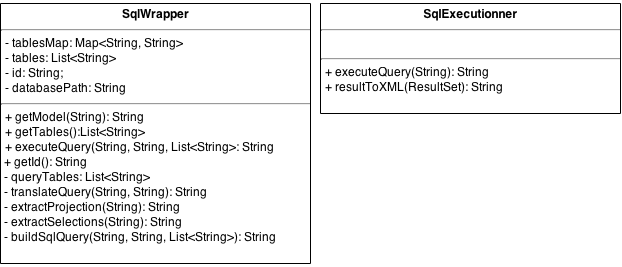
\includegraphics{WrapperSQL.png}
    \caption{Implémentation du wrapper SQL}
    \label{fig:wrapperSQL}
\end{figure}

Dans les requêtes XPath, nous avons réduit les formes sous lesquelles les projections peuvent se présenter. Nous avons gardé les cas suivants :
\begin{itemize}
\item \emph{/tuple} ou \emph{//tuple} : Pour toutes les tables SQL, nous avons ajouté un noeud \(tuple\) qui représente une ligne. Ainsi les requêtes XPath précédentes reviennent à demander toutes les lignes de la table.
\item \emph{/tuple/XXX} ou \emph{//XXX} : Les requêtes précédentes permettent d'effectuer une projection sur une des colonnes de la table \(XXX\).
\end{itemize}

Les cas présentés ci-dessus sont les seuls cas que nous avons considérés. Ainsi, il n'est pas possible de faire une projection sur plusieurs colonnes des tables SQL.


Les sélections sur le XPath ont également été gérées de façon simplifiées. Nous avons choisi de récuperer le contenu des séléctions du XPath (entre crochets) mots pour mots, et de les placer dans la partie \(WHERE\) de la requête SQL. La seule modification apportée au contenu de la sélection a été le remplacement des \(.\) par le nom de la colonne correspondante. Ce cas est illustré dans l'exemple de la \fref{ex:XPathToSql}. Dans l'éventualité ou plusieurs sélections sont présentes dans la requête XPath, nous avons choisi de les concaténer simplement avec un \(AND\).

\begin{figure}[ht!]
\begin{minted}[mathescape,linenos,numbersep=5pt,gobble=2,frame=lines,framesep=2mm]{text}
   Requete XPath sur la table Personnages :
   /tuple[nom="Simba" OR nom="Zazu"]/age[.<21]
  
   Requete SQL obtenue :
   SELECT age FROM Personnages WHERE (nom="Simba" OR nom="Zazu") AND (age<21);
\end{minted}
\caption{Exemple de transformation d'une requête XPath en requête SQL}
\label{ex:XPathToSql}
\end{figure}

\FloatBarrier
\paragraph{SQL vers XML}~~\\

Une fois la requête formée, nous avons choisi de déléguer son exécution à une seconde classe, \emph{SqlExecutionner} (\fref{fig:wrapperSQL}). Cette classe utilitaire comprend simplement une méthode d'exécution de requête SQL et une méthode de transformation d'un \(ResultSet\) en XML.

Pour l'exécution des requêtes SQL, nous avons utilisé Java DataBase Connectivity (JDBC). Cet ensemble de classes permet, de se connecter et interagir en Java avec des bases de données. Le wrapper, après avoir traduit la requête XPath en SQL, se connecte à la base de donnée concernée grâce au driver JDBC correspondant au type de la base de données, un driver SQLite dans notre cas.

Le format de retour du wrapper SQL est globalement le même que celui du wrapper XML. La différence vient du format d'une base de données SQL, dans laquelle les données sont stockées en lignes. Nous avons donc ajouté le noeud \(tuple\) qui représente cette ligne. Dès qu'une requête fait une projection sur deux colonnes ou plus, ce noeud est ajouté au retour. La \fref{lst:retourTuple} montre un exemple de retour du wrapper SQL.

\begin{figure}[ht!]
\begin{minted}[mathescape,linenos,numbersep=5pt,gobble=2,frame=lines,framesep=2mm]{xml}
   <res>
      <tuple>
         <nom>Cendrillon</nom>
         <emploi>Princesse</emploi>
      </tuple>
      <tuple>
         <nom>Simba</nom>
         <emploi>Roi Lion</emploi>
      </tuple>
   </res>
\end{minted}
\caption{Exemple de résultat pour une requête affichant les noms et emplois des individus d'un document}
\label{lst:retourTuple}
\end{figure}

L'exécution d'une requête par un driver JDBC produit en retour un objet \(ResultSet\). Pour obtenir le format décrit dans l'example de la \fref{lst:retourTuple}, nous utilisons les métadonnées de ce \(ResultSet\). Elles comprennent entre autres le nombre de colonnes et leurs noms. Nous nous servons de ces informations pour parcourir le résultat, en ajoutant les balises comprenant le nom des colonnes.


%%%%%%%%%%%%%%%%%%%%%%%%%%%%%%%%%%%%%%%%%%


\subsection{Modèle de la base fédérée}

Pour faire des requêtes sur la base, l'utilisateur a besoin de connaître l'architecture de cette dernière. 
Pour cela, une fonction permet d'accéder à la DTD des différents documents présents dans la base fédérée.
La génération de la DTD ne constituant pas le coeur de notre application et étant sujet à de nombreux cas particuliers, nous avons préféré nous tourner vers une solution robuste et déjà testée.
Nous avons ainsi choisi le module DTDGenerator issu de la librairie Saxon. 
Son utilisation est des plus directes puisqu'elle prend un document XML en entrée et rédige la DTD résultante.

La DTD définit la structure d'un document XML.
Cependant toutes les données ne sont pas stockées dans le format XML.
Dans le cas des tables SQL, nous exécutons une requête SQL sur la table de la forme \emph{SELECT * FROM MA\_TABLE LIMIT 2}.
Ensuite, nous transformons le résultat de la requête dans un format XML puis nous générons notre DTD sur le document XML.




%%%%%%%%%%%%%%%%%%%%%%%%%%%%%%%%%%%%%%%%%%
%%%%%%%%%%%%%% Exemples %%%%%%%%%%%%%%%%%%
%%%%%%%%%%%%%%%%%%%%%%%%%%%%%%%%%%%%%%%%%%


\newpage
\section{Tests}

Pour nos tests, nous nous sommes concentrés sur l'apect fonctionnel de notre solution. Ainsi, nous n'avons testé ni les performances de notre solution, ni sa résistance à une forte charge.

\subsection{Présentation de la base de test}

Notre jeu de test se constitue de quatre bases, deux au format XML et deux au format SQL. Les deux bases XML sont contenues dans deux fichiers distincts, \textit{bar.xml} et \textit{alcool.xml}, tandis que les bases SQL ne constituent qu'un seul fichier, \textit{individu.sql}. La définition précise de chaque base (au format DTD) est présente en annexe \ref{lst:modeleBDDs}.

\begin{itemize}
\item La première table XML, \textit{bar}, contient des informations sur des bars (au sens débits de boissons). Pour chaque bar, on peut trouver son nom, son adresse, la liste des alcools qui y sont servis et la liste des clients qui le fréquentent.
\item La seconde table XML, \textit{alcool}, permet de connaître les caractéristiques de différentes boissons, telles que leur nom, leur date de production, leur catégorie, leur fournisseur, ou encore leur prix.
\item Ensuite, \textit{fournisseur} est la première de nos deux tables SQL. Elle contient des informations sur les fournisseurs d'alcool, telles que leur nom, leur adresse, ou encore une description sommaire de leur activité.
\item Enfin, la deuxième base SQL, \textit{client}, décrit les diférents clients. Un client est défini par son nom, son adresse, et sa boisson favorite.
\end{itemize}


\subsection{Exemples}

Nous avons recensé dans cette partie plusieurs des tests que nous avons effectué pour vérifier le bon fonctionnement de notre solution. Bien entendu, cette liste est loin d'être exhaustive, elle a plutôt pour but de donner un aperçu des différents cas qui peuvent être rencontrés. De nombreux autres tests ont été réalisés tout au long du développement de notre solution.

%%%
\FloatBarrier
\subsubsection{Afficher le nom de tous les bars qui se trouvent à Rennes}

Cet exemple est le plus simple : nous accédons à une seule table, au format XML. La \fref{lst:requeteTest1} représente la requête, tandis que la \fref{lst:resultatTest1} présente le résultat associé.

\begin{figure}[ht!]
\begin{minted}[mathescape,linenos,numbersep=5pt,gobble=2,frame=lines,framesep=2mm]{xml}
   <barsRennes>
   {
      for $b in doc("XMLbar")//bar
      where $b//ville = "Rennes"
      return		
         <bar>
            {data($b//@nom)}
         </bar>		
   }
   </barsRennes>
\end{minted}
\caption{Requête pour afficher le nom de tous les bars qui se trouvent à Rennes}
\label{lst:requeteTest1}
\end{figure}

\begin{figure}[ht!]
\begin{minted}[mathescape,linenos,numbersep=5pt,gobble=2,frame=lines,framesep=2mm]{xml}
   <barsRennes>
      <bar>Le Chat Noir</bar>
      <bar>La Guinguette</bar>
      <bar>La Taverne</bar>
   </barsRennes>
\end{minted}
\caption{Résultat pour la requête "afficher le nom de tous les bars qui se trouvent à Rennes"}
\label{lst:resultatTest1}
\end{figure}


%%%
\FloatBarrier
\subsubsection{Afficher le nom et l'adresse de tous les clients}

Dans cet exemple, on interroge encore une seule table, mais cette fois elle est au format SQL. La \fref{lst:requeteTest2} représente la requête, tandis que la \fref{lst:resultatTest2} présente le résultat associé.

\begin{figure}[ht!]
\begin{minted}[mathescape,linenos,numbersep=5pt,gobble=2,frame=lines,framesep=2mm]{xml}
   <listeClients>
   {
      for $c in doc("SQLclient")/tuple
      return		
         <client>
            {$c/nom, $c/adresse}
         </client>		
   }
   </listeClients>
\end{minted}
\caption{Requête pour afficher le nom et l'adresse de tous les clients}
\label{lst:requeteTest2}
\end{figure}

\begin{figure}[ht!]
\begin{minted}[mathescape,linenos,numbersep=5pt,gobble=2,frame=lines,framesep=2mm]{xml}
   <listeClients>
      <client>
         <nom>Benoit Travers</nom>
         <adresse>13 rue du Morpion, Rennes</adresse>
      </client>
      <client>
         <nom>Thomas Francois</nom>
         <adresse>4 allee Sansfond, Marseille</adresse>
      </client>
      ...
   </listeClients>
\end{minted}
\caption{Résultat pour la requête "afficher le nom et l'adresse de tous les clients"}
\label{lst:resultatTest2}
\end{figure}

%%%
\FloatBarrier
\subsubsection{Afficher le nom de tous les bars qui vendent de l'alcool produit en 2014}

Ici, la requête porte sur deux tables, toutes deux au format XML et présentes dans des fichiers différents. La \fref{lst:requeteTest3} représente la requête, tandis que la \fref{lst:resultatTest3} présente le résultat associé.

\begin{figure}[ht!]
\begin{minted}[mathescape,linenos,numbersep=5pt,gobble=2,frame=lines,framesep=2mm]{xml}
   <barsAlcool2014>
   {
      for $r in distinct-values(
         for $b in doc("XMLbar")//bar,
            $a in doc("XMLalcool")//alcool
         where $b/alcool = $a/@id
         and $a//annee = "2014"
         return 
            $b/@nom )
      return <bar>{$r}</bar>
   }
   </barsAlcool2014>
\end{minted}
\caption{Requête pour afficher le nom de tous les bars qui vendent de l'alcool produit en 2014}
\label{lst:requeteTest3}
\end{figure}

\begin{figure}[ht!]
\begin{minted}[mathescape,linenos,numbersep=5pt,gobble=2,frame=lines,framesep=2mm]{xml}
   <barsAlcool2014>
      <bar>Le bar de la fin du monde</bar>
      <bar>Chez Carlos</bar>
      <bar>Le Chat Noir</bar>
      <bar>La Guinguette</bar>
      <bar>La Taverne</bar>
   </barsAlcool2014>
\end{minted}
\caption{Résultat pour la requête "afficher le nom de tous les bars qui vendent de l'alcool produit en 2014"}
\label{lst:resultatTest3}
\end{figure}


%%%
\FloatBarrier
\subsubsection{Afficher tous les fournisseurs qui fournissent de l'alcool produit en 2014}

Dans cet exemple, on interroge deux tables, l'une au format XML et l'autre au format SQL. La \fref{lst:requeteTest4} représente la requête, tandis que la \fref{lst:resultatTest4} présente le résultat associé.

\begin{figure}[ht!]
\begin{minted}[mathescape,linenos,numbersep=5pt,gobble=2,frame=lines,framesep=2mm]{xml}
   <fournisseursAlcool2014>
   {
      for $a in doc("XMLalcool")//alcool
      where $a//annee = "2014"
      return
         for $f in doc("SQLfournisseur")/tuple
         where $f/id = $a/fournisseur
         return $f	
   }
   </fournisseursAlcool2014>
\end{minted}
\caption{Requête pour afficher tous les fournisseurs qui fournissent de l'alcool produit en 2014}
\label{lst:requeteTest4}
\end{figure}

\begin{figure}[ht!]
\begin{minted}[mathescape,linenos,numbersep=5pt,gobble=2,frame=lines,framesep=2mm]{xml}
   <fournisseursAlcool2014>
      <tuple>
         <id>2</id>
         <nom>Pastistory</nom>
         <adresse>5 avenue des Bateliers, Marseille</adresse>
         <description>Le fabricant historique de Pastis.</description>
      </tuple>
      <tuple>
         <id>3</id>
         <nom>Le Foy</nom>
         <adresse>20 avenue des Buttes de Coesmes, Rennes</adresse>
         <description>Insa POWAAA</description>
      </tuple>
   </fournisseursAlcool2014>
\end{minted}
\caption{Résultat pour la requête "afficher tous les fournisseurs qui fournissent de l'alcool produit en 2014"}
\label{lst:resultatTest4}
\end{figure}



%%%
\FloatBarrier
\subsubsection{Afficher le nombre de bars qui servent l'alcool préféré de Steven Seagal}

Enfin, dans ce dernier exemple, on interroge encore deux tables de formats différents, et on ajoute en plus un \textit{count}. La \fref{lst:requeteTest5} représente la requête, tandis que la \fref{lst:resultatTest5} présente le résultat associé.

\begin{figure}[ht!]
\begin{minted}[mathescape,linenos,numbersep=5pt,gobble=2,frame=lines,framesep=2mm]{xml}
   <barsStevenSeagal>
   {
      for $c in doc("SQLclient")/tuple
      where $c/nom = "Steven Seagal"
      return count(
         for $b in doc("XMLbar")//bar
         where $b/alcool = $c/alcool_prefere
         return $b
      )
   }
  </barsStevenSeagal>
\end{minted}
\caption{Requête pour afficher le nombre de bars qui servent l'alcool préféré de Steven Seagal}
\label{lst:requeteTest5}
\end{figure}

\begin{figure}[ht!]
\begin{minted}[mathescape,linenos,numbersep=5pt,gobble=2,frame=lines,framesep=2mm]{xml}
   <barsStevenSeagal>2</barsStevenSeagal>
\end{minted}
\caption{Résultat pour la requête "afficher le nombre de bars qui servent l'alcool préféré de Steven Seagal"}
\label{lst:resultatTest5}
\end{figure}






%%%%%%%%%%%%%%%%%%%%%%%%%%%%%%%%%%%%%%%%%%
%%%%%%%%%%%%%% Conclusion %%%%%%%%%%%%%%%%
%%%%%%%%%%%%%%%%%%%%%%%%%%%%%%%%%%%%%%%%%%
\FloatBarrier
~~\\
\newpage
\section{Conclusion}

Les tests ont donc pu montrer le bon fonctionnement général de notre solution, de l'envoi de la requête du client au format XQuery à la réponse en XML. L'accent a été mis sur la décomposition des requêtes, leur routage vers les bonnes sources de données, ainsi que l'uniformisation des wrappers XML et SQL. Cela nous à permis de comprendre l'organisation globale d'une telle architecture en se focalisant sur l'essentiel, à savoir l'accès transparent de données hétérogènes.

On peut remarquer que notre solution nous permettrait assez simplement d'étendre le système à de nouvelles sources de données distantes, notamment grâce au fait que l'utilisation de XQuery/XML en langage pivot est adapté à la conversion en d'autres formats.

En piste d'amélioration, nous pourrions envisager de traiter des requêtes XQuery plus complexes, capables par exemple d'aller écrire sur des bases distantes. De plus pour constater sa robustesse en situation réelle, nous pourrions intégrer notre projet au sein d'une application web existante et/ou avec une base de test plus complète.


\newpage
\appendix
\section{Modèles des bases de données de test}
\label{lst:modeleBDDs}

\begin{figure}[ht!]
\begin{minted}[mathescape,linenos,numbersep=5pt,gobble=2,frame=lines,framesep=2mm]{xml}
    <!-- SQLclient -->
    <!ELEMENT res ( tuple+ ) >
    <!ELEMENT tuple ( id, nom, alcool_prefere, adresse ) >
    <!ELEMENT id ( #PCDATA ) >
    <!ELEMENT nom ( #PCDATA ) >
    <!ELEMENT alcool_prefere ( #PCDATA ) >
    <!ELEMENT adresse ( #PCDATA ) >
    
    <!-- SQLfournisseur -->
    <!ELEMENT res ( tuple+ ) >
    <!ELEMENT tuple ( id, nom, adresse, description ) >
    <!ELEMENT id ( #PCDATA ) >
    <!ELEMENT nom ( #PCDATA ) >
    <!ELEMENT adresse ( #PCDATA ) >
    <!ELEMENT description ( #PCDATA ) >
    
    <!-- XMLbar -->
    <!ELEMENT bars ( bar+ ) >
    <!ELEMENT bar ( alcool+, adresse, client+ ) >
    <!ATTLIST bar id NMTOKEN #REQUIRED >
    <!ATTLIST bar nom CDATA #REQUIRED >
    <!ELEMENT alcool ( #PCDATA ) >
    <!ELEMENT adresse ( ville, rue, numero ) >
    <!ELEMENT ville ( #PCDATA ) >
    <!ELEMENT rue ( #PCDATA ) >
    <!ELEMENT numero ( #PCDATA ) >
    <!ELEMENT client ( #PCDATA ) >
    
    <!-- XMLalcool -->
    <!ELEMENT alcools ( alcool+ ) >
    <!ELEMENT alcool ( fournisseur, annee, prix, description ) >
    <!ATTLIST alcool categorie NMTOKEN #REQUIRED >
    <!ATTLIST alcool id NMTOKEN #REQUIRED >
    <!ATTLIST alcool nom CDATA #REQUIRED >
    <!ELEMENT fournisseur ( #PCDATA ) >
    <!ELEMENT annee ( #PCDATA ) >
    <!ELEMENT prix ( #PCDATA ) >
    <!ELEMENT description ( #PCDATA ) >
\end{minted}
\caption{Modèle des bases de données de tests}
\end{figure}


\end{document}


